\documentclass[10pt]{article}
\usepackage{scribe-md1}
\usepackage[usenames]{color}
\usepackage{multirow}
\usepackage[table]{xcolor}% http://ctan.org/pkg/xcolor
\usepackage{caption}


\Scribes{Hannon Queiroz, Marcos Vinícius}
\Lecturer{Carlos Frederico}
\LectureNumber{Email client - } %% vazio
\LectureDate{\today} % deixar vazio se não se refere a uma aula particular
\LectureTitle{Sistemas Operacionais} % ajustar para outros trabalhos
\Disciplina{BCC264}
\Periodo{2015/2}

\begin{document}
\MakeScribeTop

\section{Definição das tecnologias}
Para realizar o trabalho proposto, serão utilizadas as seguintes tecnologias:
\begin{itemize}
 \item Linguagem de programação: Python.
 \begin{itemize}
  \item É uma linguagem de alto nível, com diversas bibliotecas que implementam tratamento de email.
 \end{itemize}

 \item \textit{Framework} para programação \textit{web}: Django.
 \begin{itemize}
  \item Este \textit{framework} fornece abstrações necessárias para um desenvolvimento rápido e de qualidade, tratando toda a lógica comum à sistemas \textit{web} de forma transparente. 
  \item Aborda as 3 camadas do modelo ``\textit{Model, View, Controller}'' (no Django, chamado de \textit{Model, View, Template}), portanto é possível desenvolver desde a modelagem do banco de dados até a camada de apresentação no browser.
 \end{itemize}

 \item Banco de dados: PostgreSQL.
\end{itemize}

Para acessar os email, faremos o uso da biblioteca \textit{Imbox}(https://github.com/martinrusev/imbox). Com esta biblioteca, é possível recuperar emails facilmente usando filtros de data, assunto e remetente.

O agendamento no Google Calendar será feito através da API disponibilizada no Google Developers.

\section{Abordagem}
Para realizar as atividades necessárias, serão usadas threads através da biblioteca threading.
A princípio, haverá 3 threads executando paralelamente: uma para recuperar emails do Gmail, outra para recuperar emails do Yahoo. Essas duas threads irão tratar os emails e salvar as informações necessárias no banco de dados. A terceira thread será responsável por ler os emails do banco de dados e adicionar os eventos no Google Calendar.

As threads que irão recuperar os emails podem ser definidas de modo que elas verifiquem se há novos emails a cada $n$ segundos, e a thread que irá adicionar os eventos no Google Calendar irá ficar dormindo até que um novo email relevante seja recebido, e a thread responsável pelos emails irá acordar a thread que adiciona eventos no Google Calendar.

Estes passos são mostrados no diagrama da figura 1.

\begin{figure}
\label{fig:diagrama}
 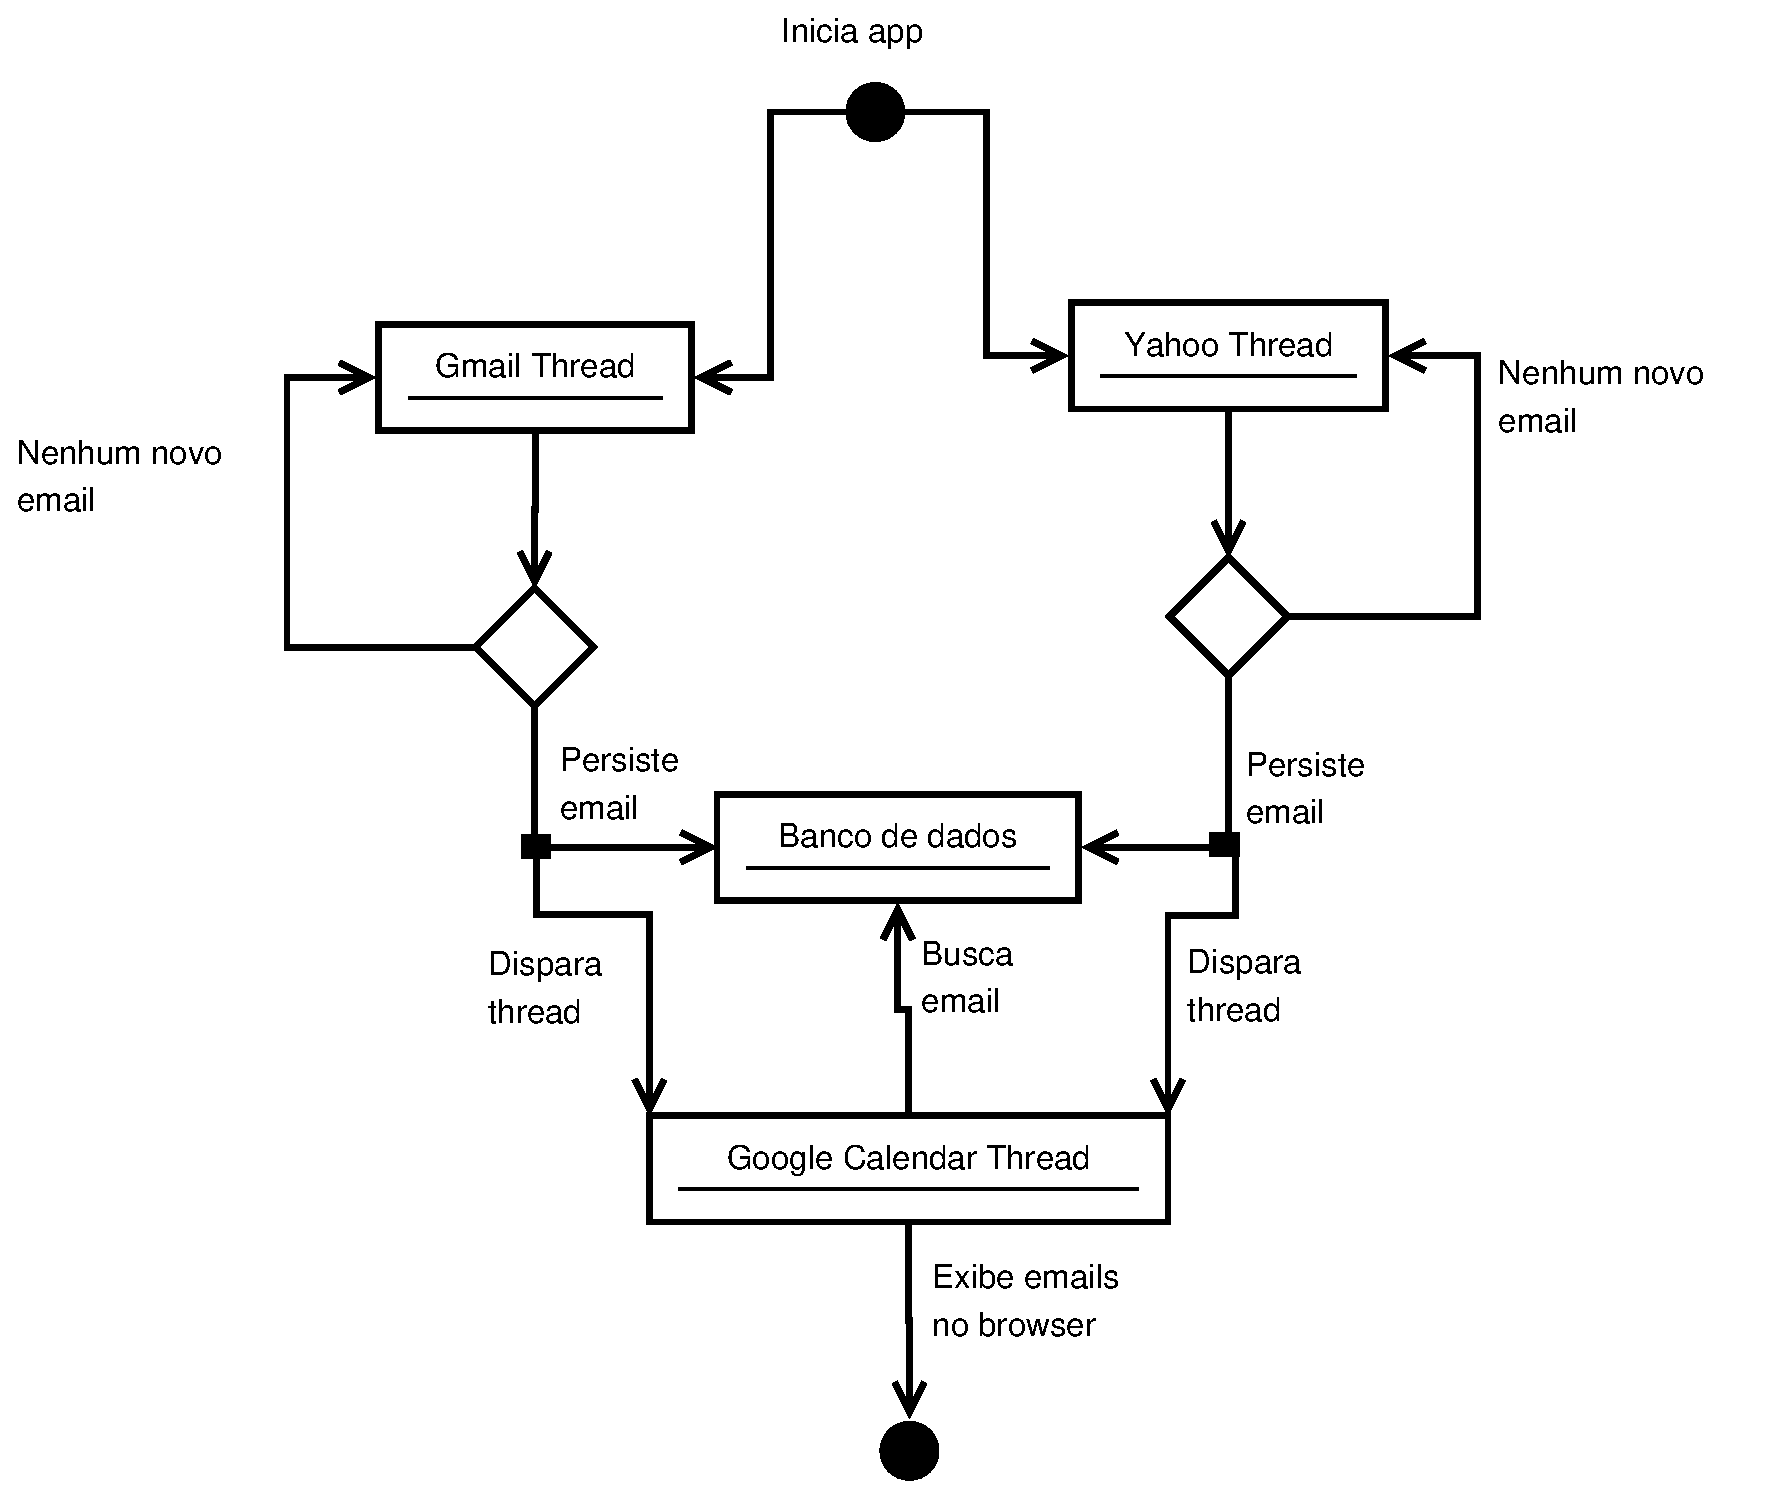
\includegraphics[scale=0.6]{diagrama}
 \caption{Diagrama do sistema}
\end{figure}



\end{document}
